% Options for packages loaded elsewhere
\PassOptionsToPackage{unicode}{hyperref}
\PassOptionsToPackage{hyphens}{url}
%
\documentclass[
]{article}
\usepackage{lmodern}
\usepackage{amssymb,amsmath}
\usepackage{ifxetex,ifluatex}
\ifnum 0\ifxetex 1\fi\ifluatex 1\fi=0 % if pdftex
  \usepackage[T1]{fontenc}
  \usepackage[utf8]{inputenc}
  \usepackage{textcomp} % provide euro and other symbols
\else % if luatex or xetex
  \usepackage{unicode-math}
  \defaultfontfeatures{Scale=MatchLowercase}
  \defaultfontfeatures[\rmfamily]{Ligatures=TeX,Scale=1}
\fi
% Use upquote if available, for straight quotes in verbatim environments
\IfFileExists{upquote.sty}{\usepackage{upquote}}{}
\IfFileExists{microtype.sty}{% use microtype if available
  \usepackage[]{microtype}
  \UseMicrotypeSet[protrusion]{basicmath} % disable protrusion for tt fonts
}{}
\makeatletter
\@ifundefined{KOMAClassName}{% if non-KOMA class
  \IfFileExists{parskip.sty}{%
    \usepackage{parskip}
  }{% else
    \setlength{\parindent}{0pt}
    \setlength{\parskip}{6pt plus 2pt minus 1pt}}
}{% if KOMA class
  \KOMAoptions{parskip=half}}
\makeatother
\usepackage{xcolor}
\IfFileExists{xurl.sty}{\usepackage{xurl}}{} % add URL line breaks if available
\IfFileExists{bookmark.sty}{\usepackage{bookmark}}{\usepackage{hyperref}}
\hypersetup{
  pdftitle={Econometrics II - Problem 6},
  pdfauthor={William Radaic Peron},
  hidelinks,
  pdfcreator={LaTeX via pandoc}}
\urlstyle{same} % disable monospaced font for URLs
\usepackage[margin=1in]{geometry}
\usepackage{color}
\usepackage{fancyvrb}
\newcommand{\VerbBar}{|}
\newcommand{\VERB}{\Verb[commandchars=\\\{\}]}
\DefineVerbatimEnvironment{Highlighting}{Verbatim}{commandchars=\\\{\}}
% Add ',fontsize=\small' for more characters per line
\usepackage{framed}
\definecolor{shadecolor}{RGB}{248,248,248}
\newenvironment{Shaded}{\begin{snugshade}}{\end{snugshade}}
\newcommand{\AlertTok}[1]{\textcolor[rgb]{0.94,0.16,0.16}{#1}}
\newcommand{\AnnotationTok}[1]{\textcolor[rgb]{0.56,0.35,0.01}{\textbf{\textit{#1}}}}
\newcommand{\AttributeTok}[1]{\textcolor[rgb]{0.77,0.63,0.00}{#1}}
\newcommand{\BaseNTok}[1]{\textcolor[rgb]{0.00,0.00,0.81}{#1}}
\newcommand{\BuiltInTok}[1]{#1}
\newcommand{\CharTok}[1]{\textcolor[rgb]{0.31,0.60,0.02}{#1}}
\newcommand{\CommentTok}[1]{\textcolor[rgb]{0.56,0.35,0.01}{\textit{#1}}}
\newcommand{\CommentVarTok}[1]{\textcolor[rgb]{0.56,0.35,0.01}{\textbf{\textit{#1}}}}
\newcommand{\ConstantTok}[1]{\textcolor[rgb]{0.00,0.00,0.00}{#1}}
\newcommand{\ControlFlowTok}[1]{\textcolor[rgb]{0.13,0.29,0.53}{\textbf{#1}}}
\newcommand{\DataTypeTok}[1]{\textcolor[rgb]{0.13,0.29,0.53}{#1}}
\newcommand{\DecValTok}[1]{\textcolor[rgb]{0.00,0.00,0.81}{#1}}
\newcommand{\DocumentationTok}[1]{\textcolor[rgb]{0.56,0.35,0.01}{\textbf{\textit{#1}}}}
\newcommand{\ErrorTok}[1]{\textcolor[rgb]{0.64,0.00,0.00}{\textbf{#1}}}
\newcommand{\ExtensionTok}[1]{#1}
\newcommand{\FloatTok}[1]{\textcolor[rgb]{0.00,0.00,0.81}{#1}}
\newcommand{\FunctionTok}[1]{\textcolor[rgb]{0.00,0.00,0.00}{#1}}
\newcommand{\ImportTok}[1]{#1}
\newcommand{\InformationTok}[1]{\textcolor[rgb]{0.56,0.35,0.01}{\textbf{\textit{#1}}}}
\newcommand{\KeywordTok}[1]{\textcolor[rgb]{0.13,0.29,0.53}{\textbf{#1}}}
\newcommand{\NormalTok}[1]{#1}
\newcommand{\OperatorTok}[1]{\textcolor[rgb]{0.81,0.36,0.00}{\textbf{#1}}}
\newcommand{\OtherTok}[1]{\textcolor[rgb]{0.56,0.35,0.01}{#1}}
\newcommand{\PreprocessorTok}[1]{\textcolor[rgb]{0.56,0.35,0.01}{\textit{#1}}}
\newcommand{\RegionMarkerTok}[1]{#1}
\newcommand{\SpecialCharTok}[1]{\textcolor[rgb]{0.00,0.00,0.00}{#1}}
\newcommand{\SpecialStringTok}[1]{\textcolor[rgb]{0.31,0.60,0.02}{#1}}
\newcommand{\StringTok}[1]{\textcolor[rgb]{0.31,0.60,0.02}{#1}}
\newcommand{\VariableTok}[1]{\textcolor[rgb]{0.00,0.00,0.00}{#1}}
\newcommand{\VerbatimStringTok}[1]{\textcolor[rgb]{0.31,0.60,0.02}{#1}}
\newcommand{\WarningTok}[1]{\textcolor[rgb]{0.56,0.35,0.01}{\textbf{\textit{#1}}}}
\usepackage{graphicx,grffile}
\makeatletter
\def\maxwidth{\ifdim\Gin@nat@width>\linewidth\linewidth\else\Gin@nat@width\fi}
\def\maxheight{\ifdim\Gin@nat@height>\textheight\textheight\else\Gin@nat@height\fi}
\makeatother
% Scale images if necessary, so that they will not overflow the page
% margins by default, and it is still possible to overwrite the defaults
% using explicit options in \includegraphics[width, height, ...]{}
\setkeys{Gin}{width=\maxwidth,height=\maxheight,keepaspectratio}
% Set default figure placement to htbp
\makeatletter
\def\fps@figure{htbp}
\makeatother
\setlength{\emergencystretch}{3em} % prevent overfull lines
\providecommand{\tightlist}{%
  \setlength{\itemsep}{0pt}\setlength{\parskip}{0pt}}
\setcounter{secnumdepth}{-\maxdimen} % remove section numbering

\title{Econometrics II - Problem 6}
\author{William Radaic Peron}
\date{\today}

\begin{document}
\maketitle

\section{Part 2: Unit roots}

As has been discussed during the lecture, when the population model is a
\emph{random walk}:
\[ Y_t = 1*Y_{t-1} + \varepsilon_t, \hspace{1em} \varepsilon \sim wn(0, \sigma^2), \]

it happens that the series \emph{is not ergodic} (nor is it stationary).
Therefore, the usual asymptotic properties \emph{do not hold}, as all
innovations have \emph{permanent effects}.
\[ Y_t = c + \delta t + \sum_{i=1}^t \varepsilon_i \]

The random walk, defined above, is an example of the more general class
of \emph{unit root processes}: \[ Y_t = c + \delta t + u_t,\]

\(u_t\) has an ARMA(p,q) representation:

\[ \Phi_p (L) u_t = \Theta_q (L) \varepsilon_t, \hspace{1em} \varepsilon \sim wn(0, \sigma^2)\]

Suppose that one of the roots of \(\Theta_p (L)\) is equal to 1:

\[ \Theta_p (L) = (1 - [1]L)(1 - \lambda_2 L)...(1 - \lambda_p L)\]

\[ (1 - L)u_t = (1 - \lambda_2 L)^{-1} ... (1 - \lambda_p L)^{-1} \Theta_q (L) \varepsilon_t =: \Psi(L) \varepsilon_t \]

We can now rewrite this as:
\[ (1- L)Y_t = (1-L)c + (1-L)\delta t + (1-L)u_t \]

\[ (1 - L)Y_t = \delta + \Psi (L) \varepsilon_t \]

Defining \(\Delta Y_t\), we have:
\[ \Delta Y_t := (1 - L)Y_t = Y_t - Y_{t-1} = \delta + \Psi (L) \varepsilon_t \]

With this concept, we can define ARIMA(p,d,q) processes:
\[ \Phi_p (L) (1-L)^d Y_t = c + \Theta_q (L) \varepsilon_t, \hspace{1em} \varepsilon_t \sim wn(0, \sigma^2) \]

\subsection{Hypothesis testing}

It turns out that testing for unit root presence presents some
challenges. Under the null (\(a_1 = 1\)), its distribution \emph{is not
standard} and does not present the usual asymptotic properties. We can
circumvent this issue with the use of numeric methods, such as the
\emph{Monte Carlo simulation}. It will now be employed, following Dickey
and Fuller (1979).

First, some notation:

We begin with a simple model: \[ Y_t = a_1 y_{t-1} + \varepsilon_t \]
\[ \Delta Y_t = \gamma y_{t-1} + \varepsilon_t, \hspace{1em} \gamma := a_1 - 1 \]
Dickey and Fuller constructed the following regression equations:
\begin{equation}
 \Delta y_t = \gamma y_{t-1} + \varepsilon_t
\end{equation}

\begin{equation}
\Delta y_t = a_0 + \gamma y_{t-1} + \varepsilon_t
\end{equation}

\begin{equation}
\Delta y_t = a_0 + \gamma y_{t-1} + a_2t + \varepsilon_t
\end{equation}

\begin{enumerate}
\def\labelenumi{(\arabic{enumi})}
\tightlist
\item
  has no intercept and represents a simple random walk. (2) includes an
  intercept. (3) also adds a deterministic time trend.
\end{enumerate}

Note that the critical values of the t-statistics are \emph{different}
between these regressions. This will now be shown with our Monte Carlo
simulation.

For equation (1):

\begin{Shaded}
\begin{Highlighting}[]
\KeywordTok{set.seed}\NormalTok{(}\DecValTok{76345}\NormalTok{)}

\CommentTok{# length of ts}
\NormalTok{T <-}\StringTok{ }\DecValTok{100}

\CommentTok{# Loops}
\NormalTok{S <-}\StringTok{ }\DecValTok{10000}

\NormalTok{e <-}\StringTok{ }\KeywordTok{rnorm}\NormalTok{(T, }\DecValTok{0}\NormalTok{, }\DecValTok{1}\NormalTok{)}

\CommentTok{# As y_\{t+1\} = y_t + \textbackslash{}varepsilon_t, we can write this as an MA(\textbackslash{}infty) model. y_t = \textbackslash{}sum \textbackslash{}varepsilon_i. This is now done with the cumsum function.}

\NormalTok{y <-}\StringTok{ }\KeywordTok{cumsum}\NormalTok{(e)}

\NormalTok{y <-}\StringTok{ }\KeywordTok{vector}\NormalTok{()}

\NormalTok{y[}\DecValTok{1}\NormalTok{] =}\StringTok{ }\NormalTok{e[}\DecValTok{1}\NormalTok{]}

\ControlFlowTok{for}\NormalTok{ (i }\ControlFlowTok{in}\NormalTok{ (}\DecValTok{2}\OperatorTok{:}\NormalTok{T)) \{}

\NormalTok{    y[i] <-}\StringTok{ }\NormalTok{y[(i}\DecValTok{-1}\NormalTok{)] }\OperatorTok{+}\StringTok{ }\NormalTok{e[i]}

\NormalTok{\}}

\NormalTok{y <-}\StringTok{ }\KeywordTok{as.ts}\NormalTok{(y)}

\KeywordTok{autoplot}\NormalTok{(y) }\OperatorTok{+}\StringTok{ }\KeywordTok{theme_bw}\NormalTok{()}
\end{Highlighting}
\end{Shaded}

\begin{center}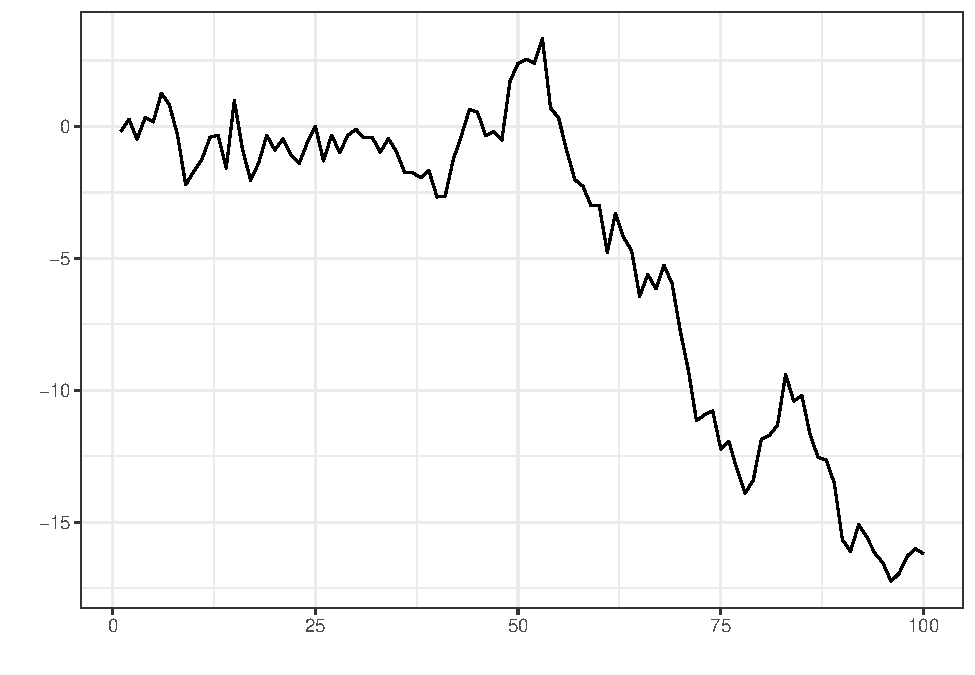
\includegraphics{Econo2_P6_files/figure-latex/monte carlo 1-1} \end{center}

\begin{Shaded}
\begin{Highlighting}[]
\CommentTok{# Taking the first difference}

\NormalTok{y_diff <-}\StringTok{ }\KeywordTok{diff}\NormalTok{(y)}

\CommentTok{# Regression of I(1) model}

\NormalTok{reg <-}\StringTok{ }\KeywordTok{dynlm}\NormalTok{(y_diff }\OperatorTok{~}\StringTok{ }\DecValTok{0} \OperatorTok{+}\StringTok{ }\KeywordTok{L}\NormalTok{(y,}\DecValTok{1}\NormalTok{)) }\CommentTok{# no lag (x1 = 0)}

\NormalTok{reg <-}\KeywordTok{summary}\NormalTok{(reg)}

\NormalTok{reg}\OperatorTok{$}\NormalTok{coefficients[}\DecValTok{1}\NormalTok{,}\DecValTok{3}\NormalTok{] }\CommentTok{# t value}
\end{Highlighting}
\end{Shaded}

\begin{verbatim}
## [1] 1.110447
\end{verbatim}

\begin{Shaded}
\begin{Highlighting}[]
\CommentTok{# Loop}

\NormalTok{tau <-}\StringTok{ }\KeywordTok{vector}\NormalTok{()}

\NormalTok{k <-}\StringTok{ }\DecValTok{1}

\NormalTok{delta <-}\StringTok{ }\DecValTok{0}

\ControlFlowTok{for}\NormalTok{ (i }\ControlFlowTok{in} \DecValTok{1}\OperatorTok{:}\NormalTok{S) \{}
  
\NormalTok{  e <-}\StringTok{ }\KeywordTok{rnorm}\NormalTok{(T,}\DecValTok{0}\NormalTok{,}\DecValTok{1}\NormalTok{)}
\NormalTok{  y =}\StringTok{ }\NormalTok{k }\OperatorTok{+}\StringTok{ }\NormalTok{delta}\OperatorTok{*}\KeywordTok{seq}\NormalTok{(}\DecValTok{1}\OperatorTok{:}\NormalTok{T) }\OperatorTok{+}\StringTok{ }\KeywordTok{cumsum}\NormalTok{(e)}
\NormalTok{  y <-}\StringTok{ }\KeywordTok{as.ts}\NormalTok{(y)}
  
\NormalTok{  y_diff <-}\StringTok{ }\KeywordTok{diff}\NormalTok{(y)}
  
\NormalTok{  reg <-}\StringTok{ }\KeywordTok{summary}\NormalTok{(}\KeywordTok{dynlm}\NormalTok{(y_diff }\OperatorTok{~}\StringTok{ }\DecValTok{1} \OperatorTok{+}\StringTok{ }\KeywordTok{L}\NormalTok{(y, }\DecValTok{1}\NormalTok{)))}
  
\NormalTok{  tau[i] <-}\StringTok{ }\NormalTok{reg}\OperatorTok{$}\NormalTok{coefficients[}\DecValTok{2}\NormalTok{,}\DecValTok{3}\NormalTok{]}
  
\NormalTok{\}}

\NormalTok{tau.df <-}\StringTok{ }\KeywordTok{data.frame}\NormalTok{(tau)}

\KeywordTok{ggplot}\NormalTok{(}\DataTypeTok{data =}\NormalTok{ tau.df, }\KeywordTok{aes}\NormalTok{(}\DataTypeTok{x =}\NormalTok{ tau)) }\OperatorTok{+}\StringTok{ }\KeywordTok{geom_density}\NormalTok{(}\DataTypeTok{color =} \StringTok{"blue"}\NormalTok{) }\OperatorTok{+}\StringTok{ }\KeywordTok{stat_function}\NormalTok{(}\DataTypeTok{fun =}\NormalTok{ dnorm, }\DataTypeTok{n =} \DecValTok{101}\NormalTok{, }\DataTypeTok{args =} \KeywordTok{c}\NormalTok{(}\DataTypeTok{mean =} \DecValTok{0}\NormalTok{, }\DataTypeTok{sd =} \DecValTok{1}\NormalTok{)) }\OperatorTok{+}\StringTok{ }\KeywordTok{theme_few}\NormalTok{()}
\end{Highlighting}
\end{Shaded}

\begin{center}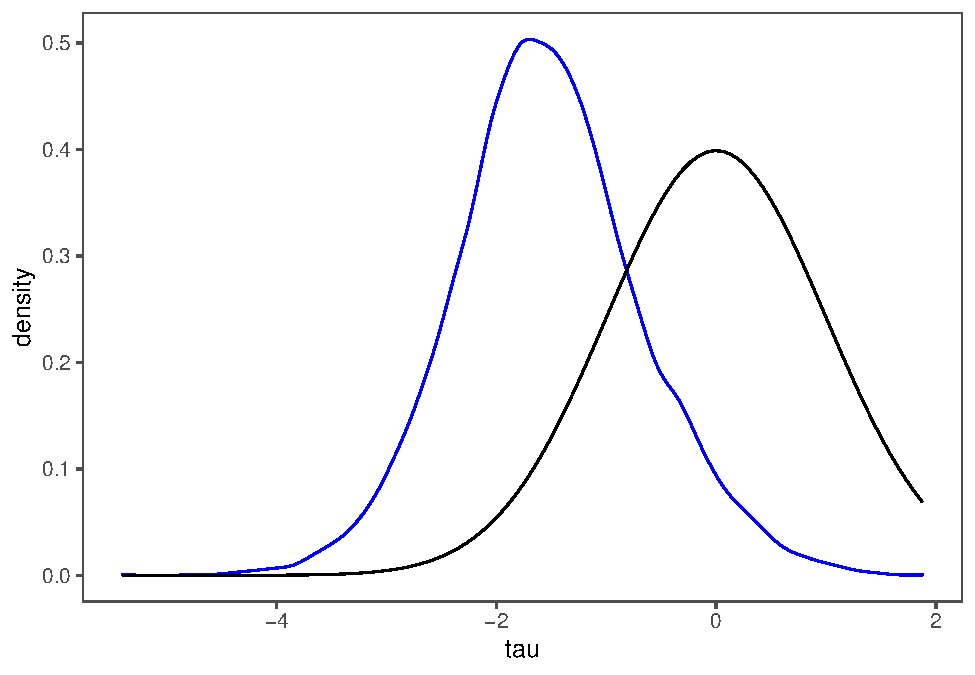
\includegraphics{Econo2_P6_files/figure-latex/monte carlo 1-2} \end{center}

\begin{Shaded}
\begin{Highlighting}[]
\KeywordTok{jarque.bera.test}\NormalTok{(tau) }\CommentTok{# We reject H0 at the 1% significance level.}
\end{Highlighting}
\end{Shaded}

\begin{verbatim}
## 
##  Jarque Bera Test
## 
## data:  tau
## X-squared = 86.138, df = 2, p-value < 2.2e-16
\end{verbatim}

\begin{Shaded}
\begin{Highlighting}[]
\NormalTok{tau.ci <-}\StringTok{ }\KeywordTok{quantile}\NormalTok{(tau, }\KeywordTok{c}\NormalTok{(}\FloatTok{0.01}\NormalTok{, }\FloatTok{0.05}\NormalTok{, }\FloatTok{0.1}\NormalTok{))}

\NormalTok{tau.ci}
\end{Highlighting}
\end{Shaded}

\begin{verbatim}
##        1%        5%       10% 
## -3.494124 -2.880240 -2.567557
\end{verbatim}

For equation (2) -- with an intercept:

\begin{Shaded}
\begin{Highlighting}[]
\CommentTok{# Loop}

\NormalTok{tau_mu <-}\StringTok{ }\KeywordTok{vector}\NormalTok{()}

\ControlFlowTok{for}\NormalTok{ (i }\ControlFlowTok{in} \DecValTok{1}\OperatorTok{:}\NormalTok{S) \{}
    
\NormalTok{    e <-}\StringTok{ }\KeywordTok{rnorm}\NormalTok{(T, }\DecValTok{0}\NormalTok{, }\DecValTok{1}\NormalTok{)}
\NormalTok{    y <-}\StringTok{ }\KeywordTok{cumsum}\NormalTok{(e)}
\NormalTok{    y <-}\StringTok{ }\KeywordTok{as.ts}\NormalTok{(y)}
    
\NormalTok{    y_diff <-}\StringTok{ }\KeywordTok{diff}\NormalTok{(y)}
    
\NormalTok{    reg <-}\StringTok{ }\KeywordTok{summary}\NormalTok{(}\KeywordTok{dynlm}\NormalTok{(y_diff }\OperatorTok{~}\StringTok{ }\DecValTok{1} \OperatorTok{+}\StringTok{ }\KeywordTok{L}\NormalTok{(y, }\DecValTok{1}\NormalTok{)))}
    
\NormalTok{    tau_mu[i] <-}\StringTok{ }\NormalTok{reg}\OperatorTok{$}\NormalTok{coefficients[}\DecValTok{2}\NormalTok{, }\DecValTok{3}\NormalTok{]}
    
\NormalTok{\}}

\NormalTok{tau_mu.df <-}\StringTok{ }\KeywordTok{data.frame}\NormalTok{(tau_mu)}

\KeywordTok{ggplot}\NormalTok{(}\DataTypeTok{data =}\NormalTok{ tau_mu.df, }\KeywordTok{aes}\NormalTok{(}\DataTypeTok{x =}\NormalTok{ tau_mu)) }\OperatorTok{+}\StringTok{ }\KeywordTok{geom_density}\NormalTok{(}\DataTypeTok{color =} \StringTok{"blue"}\NormalTok{) }\OperatorTok{+}\StringTok{ }
\StringTok{    }\KeywordTok{stat_function}\NormalTok{(}\DataTypeTok{fun =}\NormalTok{ dnorm, }\DataTypeTok{n =} \DecValTok{101}\NormalTok{, }\DataTypeTok{args =} \KeywordTok{c}\NormalTok{(}\DataTypeTok{mean =} \DecValTok{0}\NormalTok{, }\DataTypeTok{sd =} \DecValTok{1}\NormalTok{)) }\OperatorTok{+}\StringTok{ }
\StringTok{    }\KeywordTok{theme_few}\NormalTok{()}
\end{Highlighting}
\end{Shaded}

\begin{center}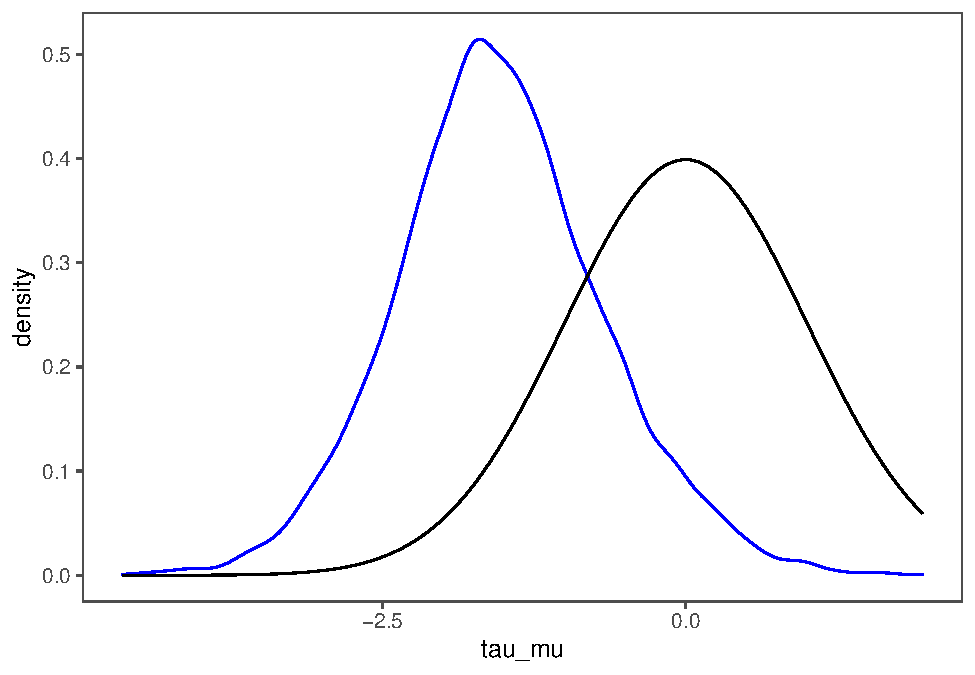
\includegraphics{Econo2_P6_files/figure-latex/monte carlo 2-1} \end{center}

\begin{Shaded}
\begin{Highlighting}[]
\KeywordTok{jarque.bera.test}\NormalTok{(tau_mu)  }\CommentTok{# We reject H0 at the 1% significance level.}
\end{Highlighting}
\end{Shaded}

\begin{verbatim}
## 
##  Jarque Bera Test
## 
## data:  tau_mu
## X-squared = 96.894, df = 2, p-value < 2.2e-16
\end{verbatim}

\begin{Shaded}
\begin{Highlighting}[]
\NormalTok{tau_mu.ci <-}\StringTok{ }\KeywordTok{quantile}\NormalTok{(tau_mu, }\KeywordTok{c}\NormalTok{(}\FloatTok{0.01}\NormalTok{, }\FloatTok{0.05}\NormalTok{, }\FloatTok{0.1}\NormalTok{))}

\NormalTok{tau_mu.ci}
\end{Highlighting}
\end{Shaded}

\begin{verbatim}
##        1%        5%       10% 
## -3.494281 -2.895757 -2.577903
\end{verbatim}

And finally, for equation (3) -- with an intercept and a deterministic
time trend:

\begin{Shaded}
\begin{Highlighting}[]
\CommentTok{# Loop}

\NormalTok{tau_t <-}\StringTok{ }\KeywordTok{vector}\NormalTok{()}
\NormalTok{time <-}\StringTok{ }\KeywordTok{c}\NormalTok{(}\DecValTok{1}\OperatorTok{:}\NormalTok{T)}

\ControlFlowTok{for}\NormalTok{ (i }\ControlFlowTok{in} \DecValTok{1}\OperatorTok{:}\NormalTok{S) \{}
    
\NormalTok{    e <-}\StringTok{ }\KeywordTok{rnorm}\NormalTok{(T, }\DecValTok{0}\NormalTok{, }\DecValTok{1}\NormalTok{)}
\NormalTok{    y <-}\StringTok{ }\KeywordTok{cumsum}\NormalTok{(e)}
\NormalTok{    y <-}\StringTok{ }\KeywordTok{as.ts}\NormalTok{(y)}
    
\NormalTok{    y_diff <-}\StringTok{ }\KeywordTok{diff}\NormalTok{(y)}
    
\NormalTok{    reg <-}\StringTok{ }\KeywordTok{summary}\NormalTok{(}\KeywordTok{dynlm}\NormalTok{(y_diff }\OperatorTok{~}\StringTok{ }\DecValTok{1} \OperatorTok{+}\StringTok{ }\KeywordTok{L}\NormalTok{(y, }\DecValTok{1}\NormalTok{) }\OperatorTok{+}\StringTok{ }\NormalTok{time[}\OperatorTok{-}\DecValTok{1}\NormalTok{]))  }\CommentTok{# removed 1 dimension for no. of obs. }
    
\NormalTok{    tau_t[i] <-}\StringTok{ }\NormalTok{reg}\OperatorTok{$}\NormalTok{coefficients[}\DecValTok{2}\NormalTok{, }\DecValTok{3}\NormalTok{]}
    
\NormalTok{\}}

\NormalTok{tau_t.df <-}\StringTok{ }\KeywordTok{data.frame}\NormalTok{(tau_t)}

\KeywordTok{ggplot}\NormalTok{(}\DataTypeTok{data =}\NormalTok{ tau_t.df, }\KeywordTok{aes}\NormalTok{(}\DataTypeTok{x =}\NormalTok{ tau_t)) }\OperatorTok{+}\StringTok{ }\KeywordTok{geom_density}\NormalTok{(}\DataTypeTok{color =} \StringTok{"blue"}\NormalTok{) }\OperatorTok{+}\StringTok{ }
\StringTok{    }\KeywordTok{stat_function}\NormalTok{(}\DataTypeTok{fun =}\NormalTok{ dnorm, }\DataTypeTok{n =} \DecValTok{101}\NormalTok{, }\DataTypeTok{args =} \KeywordTok{c}\NormalTok{(}\DataTypeTok{mean =} \DecValTok{0}\NormalTok{, }\DataTypeTok{sd =} \DecValTok{1}\NormalTok{)) }\OperatorTok{+}\StringTok{ }
\StringTok{    }\KeywordTok{theme_few}\NormalTok{()}
\end{Highlighting}
\end{Shaded}

\begin{center}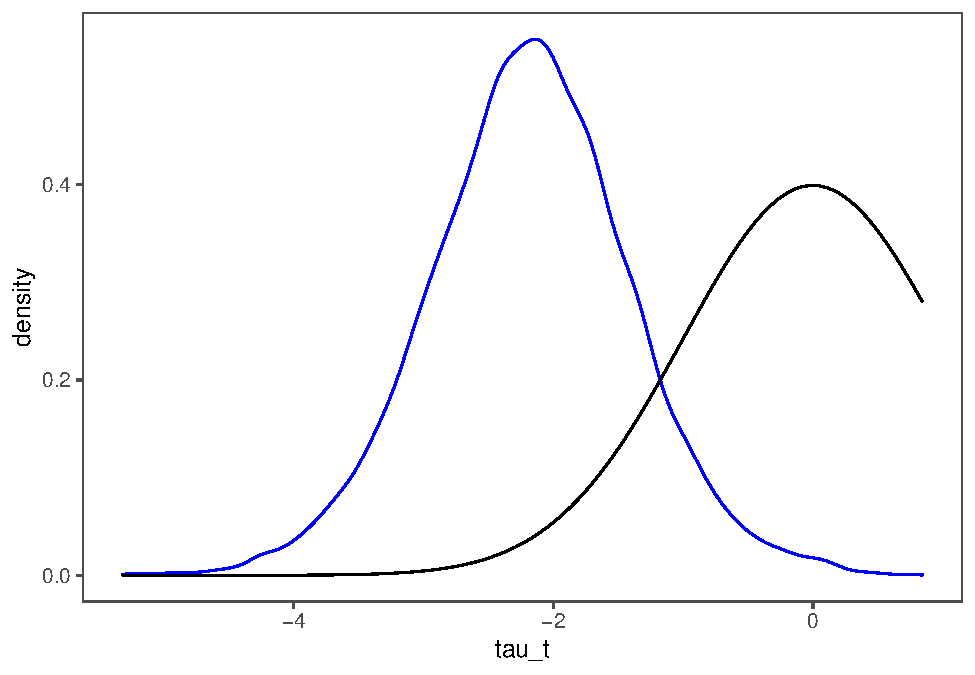
\includegraphics{Econo2_P6_files/figure-latex/monte carlo 3-1} \end{center}

\begin{Shaded}
\begin{Highlighting}[]
\KeywordTok{jarque.bera.test}\NormalTok{(tau_t)  }\CommentTok{# We reject H0 at the 1% significance level.}
\end{Highlighting}
\end{Shaded}

\begin{verbatim}
## 
##  Jarque Bera Test
## 
## data:  tau_t
## X-squared = 58.223, df = 2, p-value = 2.275e-13
\end{verbatim}

\begin{Shaded}
\begin{Highlighting}[]
\NormalTok{tau_t.ci <-}\StringTok{ }\KeywordTok{quantile}\NormalTok{(tau_t, }\KeywordTok{c}\NormalTok{(}\FloatTok{0.01}\NormalTok{, }\FloatTok{0.05}\NormalTok{, }\FloatTok{0.1}\NormalTok{))}

\NormalTok{tau_t.ci}
\end{Highlighting}
\end{Shaded}

\begin{verbatim}
##        1%        5%       10% 
## -4.065067 -3.462447 -3.158227
\end{verbatim}

Let's now change the distributions of the errors for equation (3):

\begin{Shaded}
\begin{Highlighting}[]
\CommentTok{# Loop}

\NormalTok{tau_t_pois <-}\StringTok{ }\KeywordTok{vector}\NormalTok{()}
\NormalTok{time <-}\StringTok{ }\KeywordTok{c}\NormalTok{(}\DecValTok{1}\OperatorTok{:}\NormalTok{T)}

\ControlFlowTok{for}\NormalTok{ (i }\ControlFlowTok{in} \DecValTok{1}\OperatorTok{:}\NormalTok{S) \{}
    
\NormalTok{    e <-}\StringTok{ }\KeywordTok{rpois}\NormalTok{(T, }\DecValTok{1}\NormalTok{)}
\NormalTok{    y <-}\StringTok{ }\KeywordTok{cumsum}\NormalTok{(e)}
\NormalTok{    y <-}\StringTok{ }\KeywordTok{as.ts}\NormalTok{(y)}
    
\NormalTok{    y_diff <-}\StringTok{ }\KeywordTok{diff}\NormalTok{(y)}
    
\NormalTok{    reg <-}\StringTok{ }\KeywordTok{summary}\NormalTok{(}\KeywordTok{dynlm}\NormalTok{(y_diff }\OperatorTok{~}\StringTok{ }\DecValTok{1} \OperatorTok{+}\StringTok{ }\KeywordTok{L}\NormalTok{(y, }\DecValTok{1}\NormalTok{) }\OperatorTok{+}\StringTok{ }\NormalTok{time[}\OperatorTok{-}\DecValTok{1}\NormalTok{]))  }\CommentTok{# removed 1 dimension for no. of obs. }
    
\NormalTok{    tau_t_pois[i] <-}\StringTok{ }\NormalTok{reg}\OperatorTok{$}\NormalTok{coefficients[}\DecValTok{2}\NormalTok{, }\DecValTok{3}\NormalTok{]}
    
\NormalTok{\}}

\NormalTok{tau_t_pois.df <-}\StringTok{ }\KeywordTok{data.frame}\NormalTok{(tau_t_pois)}

\KeywordTok{ggplot}\NormalTok{(}\DataTypeTok{data =}\NormalTok{ tau_t_pois.df, }\KeywordTok{aes}\NormalTok{(}\DataTypeTok{x =}\NormalTok{ tau_t_pois)) }\OperatorTok{+}\StringTok{ }\KeywordTok{geom_density}\NormalTok{(}\DataTypeTok{color =} \StringTok{"blue"}\NormalTok{) }\OperatorTok{+}\StringTok{ }
\StringTok{    }\KeywordTok{stat_function}\NormalTok{(}\DataTypeTok{fun =}\NormalTok{ dnorm, }\DataTypeTok{n =} \DecValTok{101}\NormalTok{, }\DataTypeTok{args =} \KeywordTok{c}\NormalTok{(}\DataTypeTok{mean =} \DecValTok{0}\NormalTok{, }\DataTypeTok{sd =} \DecValTok{1}\NormalTok{)) }\OperatorTok{+}\StringTok{ }
\StringTok{    }\KeywordTok{theme_few}\NormalTok{()}
\end{Highlighting}
\end{Shaded}

\begin{center}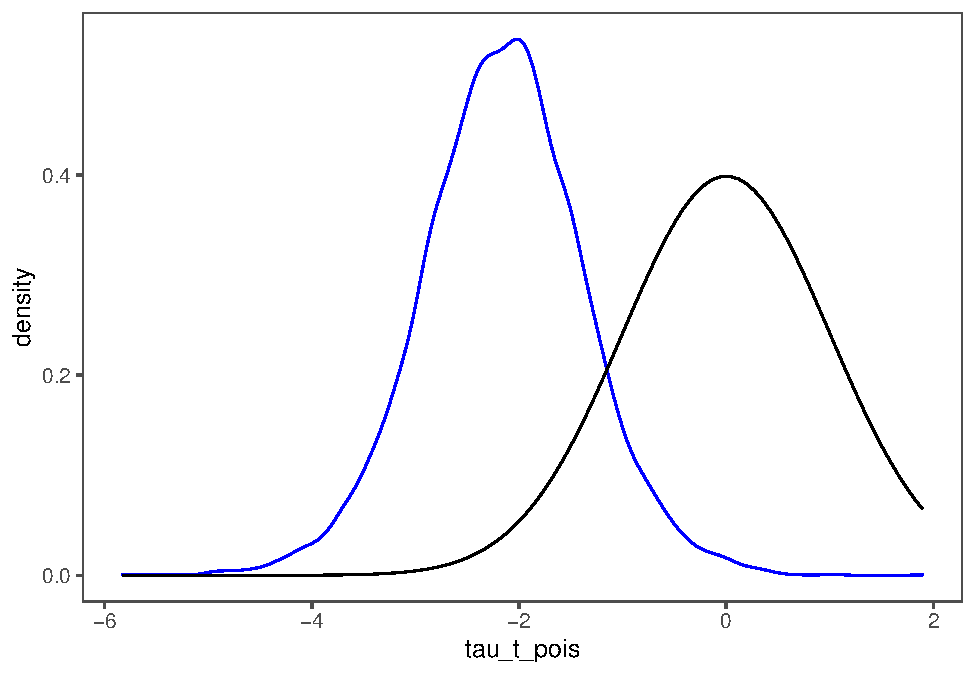
\includegraphics{Econo2_P6_files/figure-latex/monte carlo poisson-1} \end{center}

\begin{Shaded}
\begin{Highlighting}[]
\KeywordTok{jarque.bera.test}\NormalTok{(tau_t_pois)  }\CommentTok{# We reject H0 at the 1% significance level.}
\end{Highlighting}
\end{Shaded}

\begin{verbatim}
## 
##  Jarque Bera Test
## 
## data:  tau_t_pois
## X-squared = 120.61, df = 2, p-value < 2.2e-16
\end{verbatim}

\begin{Shaded}
\begin{Highlighting}[]
\NormalTok{tau_t_pois.ci <-}\StringTok{ }\KeywordTok{quantile}\NormalTok{(tau_t_pois, }\KeywordTok{c}\NormalTok{(}\FloatTok{0.01}\NormalTok{, }\FloatTok{0.05}\NormalTok{, }\FloatTok{0.1}\NormalTok{))}

\NormalTok{tau_t_pois.ci}
\end{Highlighting}
\end{Shaded}

\begin{verbatim}
##        1%        5%       10% 
## -4.085753 -3.436365 -3.127525
\end{verbatim}

\section{Part 3: Applying the Dickey-Fuller test for GDP}

Loading the data from the previous problem:

\begin{Shaded}
\begin{Highlighting}[]
\NormalTok{pib <-}\StringTok{ }\KeywordTok{get_sidra}\NormalTok{(}\DecValTok{6612}\NormalTok{, }\DataTypeTok{variable =} \DecValTok{9318}\NormalTok{, }\DataTypeTok{category =} \DecValTok{90707}\NormalTok{, }\DataTypeTok{period =} \StringTok{"all"}\NormalTok{)}
\end{Highlighting}
\end{Shaded}

\begin{verbatim}
## Considering all categories once 'classific' was set to 'all' (default)
\end{verbatim}

\begin{Shaded}
\begin{Highlighting}[]
\NormalTok{pib_limpo <-}\StringTok{ }\NormalTok{pib[(pib}\OperatorTok{$}\StringTok{`}\DataTypeTok{Setores e subsetores (Código)}\StringTok{`} \OperatorTok{==}\StringTok{ }\DecValTok{90707}\NormalTok{), }
\NormalTok{    ]}

\NormalTok{pib <-}\StringTok{ }\NormalTok{pib_limpo}

\NormalTok{pib_limpo2 <-}\StringTok{ }\NormalTok{pib[, }\KeywordTok{c}\NormalTok{(}\DecValTok{5}\NormalTok{, }\DecValTok{13}\NormalTok{)]}

\NormalTok{pib <-}\StringTok{ }\NormalTok{pib_limpo2}

\KeywordTok{names}\NormalTok{(pib)[}\DecValTok{1}\NormalTok{] <-}\StringTok{ "t"}
\KeywordTok{names}\NormalTok{(pib)[}\DecValTok{2}\NormalTok{] <-}\StringTok{ "v"}

\NormalTok{pib}\OperatorTok{$}\NormalTok{t <-}\StringTok{ }\KeywordTok{as.numeric}\NormalTok{(pib}\OperatorTok{$}\NormalTok{t)}

\KeywordTok{names}\NormalTok{(pib)}
\end{Highlighting}
\end{Shaded}

\begin{verbatim}
## [1] "t" "v"
\end{verbatim}

\begin{Shaded}
\begin{Highlighting}[]
\KeywordTok{head}\NormalTok{(pib)}
\end{Highlighting}
\end{Shaded}

\begin{verbatim}
##          t        v
## 18  199601 170920.0
## 40  199602 176708.8
## 62  199603 189844.3
## 84  199604 184112.9
## 106 199701 176732.2
## 128 199702 185109.5
\end{verbatim}

\begin{Shaded}
\begin{Highlighting}[]
\KeywordTok{tail}\NormalTok{(pib)}
\end{Highlighting}
\end{Shaded}

\begin{verbatim}
##           t        v
## 2042 201901 292647.6
## 2064 201902 297748.9
## 2086 201903 305150.9
## 2108 201904 302108.7
## 2130 202001 291912.5
## 2152 202002 263699.7
\end{verbatim}

\begin{Shaded}
\begin{Highlighting}[]
\NormalTok{pib <-}\StringTok{ }\KeywordTok{ts}\NormalTok{(pib}\OperatorTok{$}\NormalTok{v)}
\end{Highlighting}
\end{Shaded}

\begin{Shaded}
\begin{Highlighting}[]
\CommentTok{# Choosing the correct model with auto.arima}

\NormalTok{aa_pib <-}\StringTok{ }\KeywordTok{auto.arima}\NormalTok{(pib, }\DataTypeTok{stepwise =}\NormalTok{ F)}

\KeywordTok{summary}\NormalTok{(aa_pib)}
\end{Highlighting}
\end{Shaded}

\begin{verbatim}
## Series: pib 
## ARIMA(2,1,2) with drift 
## 
## Coefficients:
##           ar1      ar2     ma1    ma2     drift
##       -0.0092  -0.9764  0.2721  0.956  864.9855
## s.e.   0.0233   0.0171  0.0455  0.117  537.6284
## 
## sigma^2 estimated as 23455415:  log likelihood=-961.03
## AIC=1934.06   AICc=1934.99   BIC=1949.51
## 
## Training set error measures:
##                    ME    RMSE      MAE        MPE     MAPE      MASE       ACF1
## Training set 64.56963 4692.48 3219.806 0.05416274 1.322955 0.5203698 0.01746157
\end{verbatim}

\emph{auto.arima} yields an ARIMA(2,1,2) model with a drift parameter:
\[ \Delta y_t = a_0 + a_1 \Delta y_{t-1} + a_2 \Delta y_{t-2} + a_3 \Delta \varepsilon_{t-1} + a_4 \Delta \varepsilon_{t-2} +\varepsilon_t \]

Let's decompose this process. First, we'll perform the Dickey-Fuller
test on the GDP ts.

\begin{Shaded}
\begin{Highlighting}[]
\KeywordTok{adf.test}\NormalTok{(pib)}
\end{Highlighting}
\end{Shaded}

\begin{verbatim}
## Warning in adf.test(pib): p-value greater than printed p-value
\end{verbatim}

\begin{verbatim}
## 
##  Augmented Dickey-Fuller Test
## 
## data:  pib
## Dickey-Fuller = 0.12028, Lag order = 4, p-value = 0.99
## alternative hypothesis: stationary
\end{verbatim}

As we have not been able to reject \(H_0\), it follows that the ts
includes (at least one) unit root. Now, let's find the optimal model for
the regression.

\begin{Shaded}
\begin{Highlighting}[]
\NormalTok{max_p <-}\StringTok{ }\DecValTok{5}

\NormalTok{max_q <-}\StringTok{ }\DecValTok{5}

\NormalTok{max_d <-}\StringTok{ }\DecValTok{2}

\NormalTok{models1 <-}\StringTok{ }\KeywordTok{vector}\NormalTok{(}\StringTok{"list"}\NormalTok{, (max_p }\OperatorTok{+}\StringTok{ }\DecValTok{1}\NormalTok{) }\OperatorTok{*}\StringTok{ }\NormalTok{(max_q }\OperatorTok{+}\StringTok{ }\DecValTok{1}\NormalTok{))}

\NormalTok{models2 <-}\StringTok{ }\KeywordTok{vector}\NormalTok{(}\StringTok{"list"}\NormalTok{, (max_p }\OperatorTok{+}\StringTok{ }\DecValTok{1}\NormalTok{) }\OperatorTok{*}\StringTok{ }\NormalTok{(max_q }\OperatorTok{+}\StringTok{ }\DecValTok{1}\NormalTok{))}

\CommentTok{# Updating the model}

\NormalTok{fit1 <-}\StringTok{ }\KeywordTok{vector}\NormalTok{(}\StringTok{"list"}\NormalTok{, (max_p }\OperatorTok{+}\StringTok{ }\DecValTok{1}\NormalTok{) }\OperatorTok{*}\StringTok{ }\NormalTok{(max_q }\OperatorTok{+}\StringTok{ }\DecValTok{1}\NormalTok{))}

\NormalTok{fit2 <-}\StringTok{ }\KeywordTok{vector}\NormalTok{(}\StringTok{"list"}\NormalTok{, (max_p }\OperatorTok{+}\StringTok{ }\DecValTok{1}\NormalTok{) }\OperatorTok{*}\StringTok{ }\NormalTok{(max_q }\OperatorTok{+}\StringTok{ }\DecValTok{1}\NormalTok{))}

\NormalTok{model_info1 <-}\StringTok{ }\KeywordTok{data.frame}\NormalTok{(}\KeywordTok{matrix}\NormalTok{(}\OtherTok{NA}\NormalTok{, }\DataTypeTok{nrow =}\NormalTok{ ((max_p }\OperatorTok{+}\StringTok{ }\DecValTok{1}\NormalTok{) }\OperatorTok{*}\StringTok{ }\NormalTok{(max_q }\OperatorTok{+}\StringTok{ }
\StringTok{    }\DecValTok{1}\NormalTok{)), }\DataTypeTok{ncol =} \DecValTok{3}\NormalTok{))}




\CommentTok{# Updating the model}

\ControlFlowTok{for}\NormalTok{ (u }\ControlFlowTok{in} \DecValTok{0}\OperatorTok{:}\NormalTok{max_q) \{}
    
    \ControlFlowTok{for}\NormalTok{ (j }\ControlFlowTok{in} \DecValTok{0}\OperatorTok{:}\NormalTok{max_p) \{}
        
        
\NormalTok{        fit1[[(((max_p }\OperatorTok{+}\StringTok{ }\DecValTok{1}\NormalTok{) }\OperatorTok{*}\StringTok{ }\NormalTok{j) }\OperatorTok{+}\StringTok{ }\NormalTok{u }\OperatorTok{+}\StringTok{ }\DecValTok{1}\NormalTok{)]] <-}\StringTok{ }\KeywordTok{Arima}\NormalTok{(pib, }\DataTypeTok{order =} \KeywordTok{c}\NormalTok{(j, }
            \DecValTok{1}\NormalTok{, u))}
        
\NormalTok{        model_info1[(((max_p }\OperatorTok{+}\StringTok{ }\DecValTok{1}\NormalTok{) }\OperatorTok{*}\StringTok{ }\NormalTok{j) }\OperatorTok{+}\StringTok{ }\NormalTok{u }\OperatorTok{+}\StringTok{ }\DecValTok{1}\NormalTok{), }\DecValTok{1}\OperatorTok{:}\DecValTok{2}\NormalTok{] <-}\StringTok{ }\KeywordTok{c}\NormalTok{(fit1[[(((max_p }\OperatorTok{+}\StringTok{ }
\StringTok{            }\DecValTok{1}\NormalTok{) }\OperatorTok{*}\StringTok{ }\NormalTok{j) }\OperatorTok{+}\StringTok{ }\NormalTok{u }\OperatorTok{+}\StringTok{ }\DecValTok{1}\NormalTok{)]]}\OperatorTok{$}\NormalTok{aic, fit1[[(((max_p }\OperatorTok{+}\StringTok{ }\DecValTok{1}\NormalTok{) }\OperatorTok{*}\StringTok{ }\NormalTok{j) }\OperatorTok{+}\StringTok{ }
\StringTok{            }\NormalTok{u }\OperatorTok{+}\StringTok{ }\DecValTok{1}\NormalTok{)]]}\OperatorTok{$}\NormalTok{bic)}
        
        
        
        
\NormalTok{    \}}
\NormalTok{\}}

\KeywordTok{names}\NormalTok{(model_info1) <-}\StringTok{ }\KeywordTok{c}\NormalTok{(}\StringTok{"AIC"}\NormalTok{, }\StringTok{"BIC"}\NormalTok{, }\StringTok{"void"}\NormalTok{)}



\KeywordTok{which.min}\NormalTok{(model_info1}\OperatorTok{$}\NormalTok{AIC)}
\end{Highlighting}
\end{Shaded}

\begin{verbatim}
## [1] 23
\end{verbatim}

\begin{Shaded}
\begin{Highlighting}[]
\KeywordTok{which.min}\NormalTok{(model_info1}\OperatorTok{$}\NormalTok{BIC)}
\end{Highlighting}
\end{Shaded}

\begin{verbatim}
## [1] 15
\end{verbatim}

\begin{Shaded}
\begin{Highlighting}[]
\NormalTok{fit1[[}\KeywordTok{which.min}\NormalTok{(model_info1}\OperatorTok{$}\NormalTok{AIC)]]}
\end{Highlighting}
\end{Shaded}

\begin{verbatim}
## Series: pib 
## ARIMA(3,1,4) 
## 
## Coefficients:
##           ar1      ar2      ar3     ma1     ma2     ma3     ma4
##       -0.9688  -0.9834  -0.9685  1.4659  1.3755  1.2705  0.5008
## s.e.   0.0305   0.0210   0.0270  0.1344  0.1682  0.1821  0.1484
## 
## sigma^2 estimated as 21987482:  log likelihood=-956.26
## AIC=1928.53   AICc=1930.17   BIC=1949.13
\end{verbatim}

\begin{Shaded}
\begin{Highlighting}[]
\NormalTok{fit1[[}\KeywordTok{which.min}\NormalTok{(model_info1}\OperatorTok{$}\NormalTok{BIC)]]}
\end{Highlighting}
\end{Shaded}

\begin{verbatim}
## Series: pib 
## ARIMA(2,1,2) 
## 
## Coefficients:
##           ar1      ar2     ma1     ma2
##       -0.0084  -0.9757  0.2769  0.9673
## s.e.   0.0236   0.0175  0.0408  0.1130
## 
## sigma^2 estimated as 23692560:  log likelihood=-962.3
## AIC=1934.6   AICc=1935.26   BIC=1947.47
\end{verbatim}

\begin{Shaded}
\begin{Highlighting}[]
\CommentTok{# For I(2)}

\NormalTok{model_info2 <-}\StringTok{ }\KeywordTok{data.frame}\NormalTok{(}\KeywordTok{matrix}\NormalTok{(}\OtherTok{NA}\NormalTok{, }\DataTypeTok{nrow =}\NormalTok{ max_d }\OperatorTok{*}\StringTok{ }\NormalTok{((max_p }\OperatorTok{+}\StringTok{ }
\StringTok{    }\DecValTok{1}\NormalTok{) }\OperatorTok{*}\StringTok{ }\NormalTok{(max_q }\OperatorTok{+}\StringTok{ }\DecValTok{1}\NormalTok{)), }\DataTypeTok{ncol =} \DecValTok{3}\NormalTok{))}

\ControlFlowTok{for}\NormalTok{ (u }\ControlFlowTok{in} \DecValTok{0}\OperatorTok{:}\NormalTok{max_q) \{}
    
    \ControlFlowTok{for}\NormalTok{ (j }\ControlFlowTok{in} \DecValTok{0}\OperatorTok{:}\NormalTok{max_p) \{}
        
        
\NormalTok{        fit2[[(((max_p }\OperatorTok{+}\StringTok{ }\DecValTok{1}\NormalTok{) }\OperatorTok{*}\StringTok{ }\NormalTok{j) }\OperatorTok{+}\StringTok{ }\NormalTok{u }\OperatorTok{+}\StringTok{ }\DecValTok{1}\NormalTok{)]] <-}\StringTok{ }\KeywordTok{Arima}\NormalTok{(pib, }\DataTypeTok{order =} \KeywordTok{c}\NormalTok{(j, }
            \DecValTok{2}\NormalTok{, u))}
        
\NormalTok{        model_info2[(((max_p }\OperatorTok{+}\StringTok{ }\DecValTok{1}\NormalTok{) }\OperatorTok{*}\StringTok{ }\NormalTok{j) }\OperatorTok{+}\StringTok{ }\NormalTok{u }\OperatorTok{+}\StringTok{ }\DecValTok{1}\NormalTok{), }\DecValTok{1}\OperatorTok{:}\DecValTok{2}\NormalTok{] <-}\StringTok{ }\KeywordTok{c}\NormalTok{(fit2[[(((max_p }\OperatorTok{+}\StringTok{ }
\StringTok{            }\DecValTok{1}\NormalTok{) }\OperatorTok{*}\StringTok{ }\NormalTok{j) }\OperatorTok{+}\StringTok{ }\NormalTok{u }\OperatorTok{+}\StringTok{ }\DecValTok{1}\NormalTok{)]]}\OperatorTok{$}\NormalTok{aic, fit2[[(((max_p }\OperatorTok{+}\StringTok{ }\DecValTok{1}\NormalTok{) }\OperatorTok{*}\StringTok{ }\NormalTok{j) }\OperatorTok{+}\StringTok{ }
\StringTok{            }\NormalTok{u }\OperatorTok{+}\StringTok{ }\DecValTok{1}\NormalTok{)]]}\OperatorTok{$}\NormalTok{bic)}
        
\NormalTok{    \}}
\NormalTok{\}}

\KeywordTok{names}\NormalTok{(model_info2) <-}\StringTok{ }\KeywordTok{c}\NormalTok{(}\StringTok{"AIC"}\NormalTok{, }\StringTok{"BIC"}\NormalTok{, }\StringTok{"void"}\NormalTok{)}

\KeywordTok{which.min}\NormalTok{(model_info2}\OperatorTok{$}\NormalTok{AIC)}
\end{Highlighting}
\end{Shaded}

\begin{verbatim}
## [1] 24
\end{verbatim}

\begin{Shaded}
\begin{Highlighting}[]
\KeywordTok{which.min}\NormalTok{(model_info2}\OperatorTok{$}\NormalTok{BIC)}
\end{Highlighting}
\end{Shaded}

\begin{verbatim}
## [1] 16
\end{verbatim}

\begin{Shaded}
\begin{Highlighting}[]
\NormalTok{fit2[[}\KeywordTok{which.min}\NormalTok{(model_info2}\OperatorTok{$}\NormalTok{AIC)]]}
\end{Highlighting}
\end{Shaded}

\begin{verbatim}
## Series: pib 
## ARIMA(3,2,5) 
## 
## Coefficients:
##           ar1      ar2      ar3     ma1     ma2      ma3      ma4      ma5
##       -0.9700  -0.9835  -0.9674  0.4748  0.0162  -0.0121  -0.6534  -0.3766
## s.e.   0.0315   0.0218   0.0277  0.1511  0.1211   0.1508   0.1090   0.1793
## 
## sigma^2 estimated as 22148502:  log likelihood=-946.73
## AIC=1911.47   AICc=1913.56   BIC=1934.55
\end{verbatim}

\begin{Shaded}
\begin{Highlighting}[]
\NormalTok{fit2[[}\KeywordTok{which.min}\NormalTok{(model_info2}\OperatorTok{$}\NormalTok{BIC)]]}
\end{Highlighting}
\end{Shaded}

\begin{verbatim}
## Series: pib 
## ARIMA(2,2,3) 
## 
## Coefficients:
##           ar1      ar2      ma1     ma2      ma3
##       -0.0054  -0.9795  -0.6754  0.6720  -0.7903
## s.e.   0.0248   0.0162   0.1121  0.0786   0.1482
## 
## sigma^2 estimated as 23858414:  log likelihood=-951.82
## AIC=1915.63   AICc=1916.58   BIC=1931.02
\end{verbatim}

\end{document}
